\chapter{Analyzing the Study Dataset}
\label{cha:studyDataSet}

In this chapter, we explain the whole process of data extraction, focusing on the key aspects of the study dataset. Before we discuss the implementation and results, it's important to understand the preparation process, the distributions of the data features and their entropy. It is crucial to identify the main features, and talk about why certain features are more important and were included but others not.

\section{Data Preparation and Preprocessing}

The structure of the study dataset closely resembles that described in chapter ~\ref{cha:exampleDataset}. Consequently, the initial approach was once again identical. We began by converting the XML file into a CSV table before proceeding with further preparations. 

We have two XML files that are available to us. One is the 'export.xml' file and the other is the 'export\_cda.xml' file. First, we convert both into CSV tables and then consider whether we want to use both. After a closer look, we realize that in the clinical document architecture (CDA) document, the first five of the ten columns have identical entries per column throughout. We therefore consider these to be unusable but used the columns 'DisplayName', 'MeasurementValue', 'Unit' and 'EffectiveTime'. The mentioned CDA columns, contain information on the height, weight and heart rates of the test subjects. The information is also provided with a time stamp, which makes it easier to ensure a comparison with the other data and to simplify the subsequent merging of the tables. 

The converted export file, on the other hand, consists of 36 columns. Of the 36 columns, 29 are empty and therefore unusable. The remaining columns provide information such as 'type', 'value', 'unit', 'startDate', 'endDate', and 'creationDate', as mentioned in chapter ~\ref{cha:exampleDataset}. We therefore re-extracted the table and removed all columns except for the six aforementioned ones.

In addition to the 'export' and 'export\_cda' files, we were given access to a Google shared document titled '6MWT\_Test\_Runs'. In this document, a study supervisor documented important information during the data collection process. This provided us with essential details such as the 'study ID', 'height', 'weight', 'age', 'leg length', and entries in the 'Subject/Patient' column, indicating whether the participant was healthy or a patient. Additionally, the document contains information about all other electronic devices used for the measurements and the data they collected. However, we focused exclusively on data related to the Apple Watch Ultra. Specifically, we filtered and utilized the columns 'Distance (km)', 'Steps (before)', 'Steps (after)', and 'Steps'. The shared document consists of four relevant sheets.

Next, we needed to merge the export file with the '6MWT\_Test\_Runs' document to make the most of all available and relevant information. We initially looked for a unique function to combine the tables effectively. Despite several attempts, this approach was unsuccessful. Eventually, we found that the combination of height, weight and the time stamp served as the best criteria for merging the datasets. This process was done manually since the shared document recorded height and weight with precise decimal values, whereas the Apple Watch Ultra rounded these.

We ensured accuracy by verifying that entries in the shared document were recorded chronologically, starting with the first participant and continuing in sequence, matching the temporally sorted data collected by the Apple Watch Ultra. This cross-verification allowed us to merge the tables as accurately as possible. Any participants for whom a match could not be found were removed from the dataset. This meticulous process ensured that the merged dataset was comprehensive and precise, setting a solid foundation for further analysis.

Finally, we performed fine-tuning of the dataset. Initially, we worked with three heart rate values per participant: the lowest, highest, and average heart rates. These values were sequentially added to new columns, labeled as 'Heart Rate 1' to 'Heart Rate 3'. This approach ensured that the dataset was optimally prepared for further analysis.

\subsection{Visual Heart Rate Analysis}

We selected the day with the highest heart rate for both a male and a female subject and filtered all the heart rate data from that day during the 6 MWT. This analysis resulted in the following graphs for two healthy individuals:

\FloatBarrier
\begin{figure}[h!]
  \centering
  \begin{minipage}[b]{0.8\linewidth}
    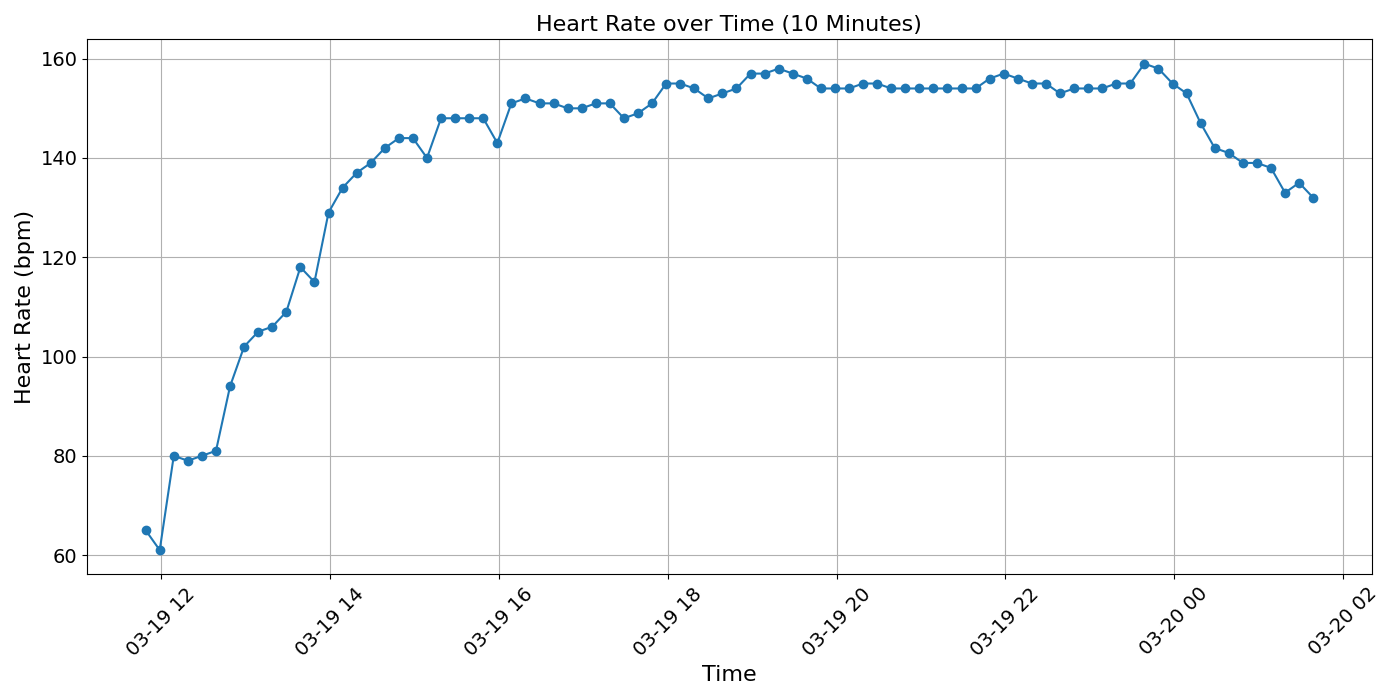
\includegraphics[width=\linewidth]{Master Thesis/Plots/HeartRate1day_Subject_male.png}
    \caption{Day of maximal heart rate in a male subject}
    \label{fig:maxheartorigmale}
  \end{minipage}
  \quad % Fügt etwas Platz zwischen den Bildern ein
  \begin{minipage}[b]{0.8\linewidth}
    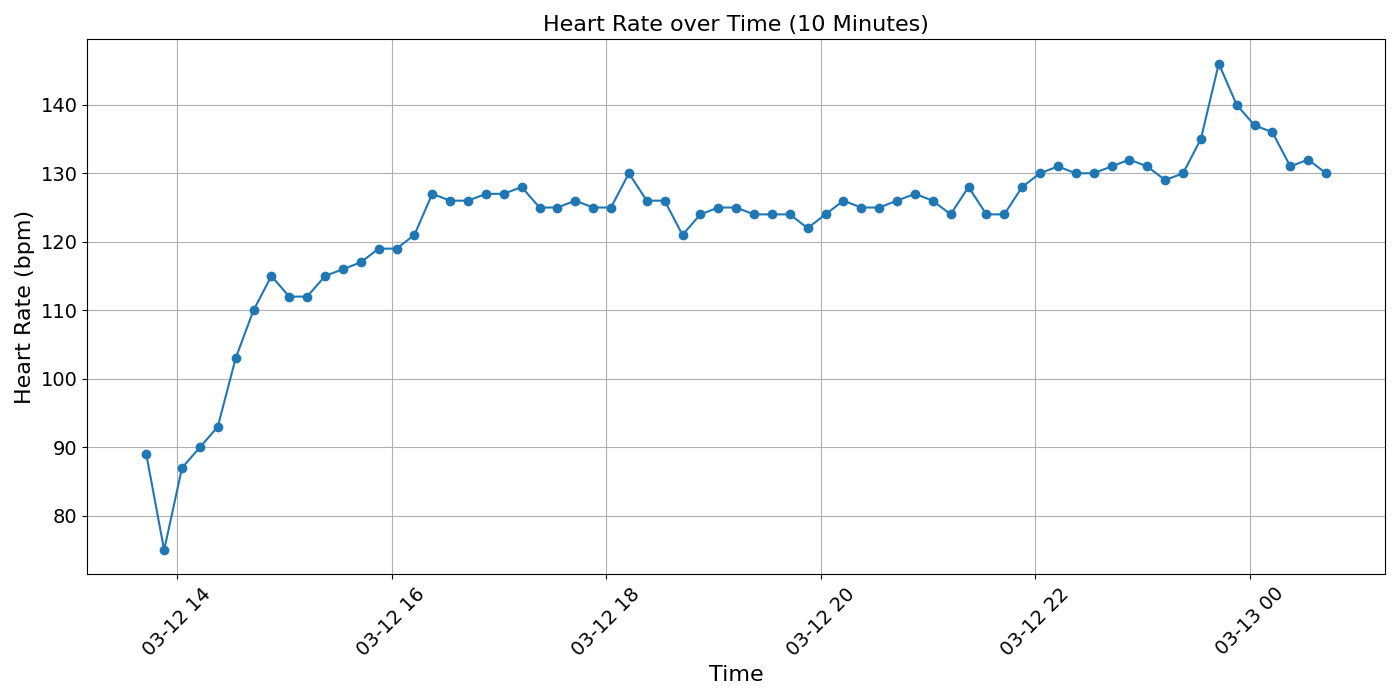
\includegraphics[width=\linewidth]{Master Thesis/Plots/HeartRate1day_Subject_female.png}
    \caption{Day of maximal heart rate in a female subject}
    \label{fig:maxheartorigfemale}
  \end{minipage}
\end{figure}
\FloatBarrier

The two figures ~\ref{fig:maxheartorigmale} and ~\ref{fig:maxheartorigfemale} displayed illustrate the heart rate variations over a 10-minute interval for two subjects, each on their day of maximal recorded heart rate, to ensure we see the heart rate before and after the 6MWT as well. These plots provide insights into the heart rate trends and highlight the differences in cardiovascular response between the subjects.

Figure ~\ref{fig:maxheartorigmale} represents the heart rate data for a male subject over 30 years of age. The heart rate starts at around 60 bpm and shows a steady increase, reaching a peak of approximately 160 bpm. After reaching the peak, the heart rate stabilizes at this high level for a while before gradually decreasing towards the end of the 10-minute interval.

Figure ~\ref{fig:maxheartorigfemale} depicts the heart rate data for a female subject over 25 years of age. The heart rate begins at around 80 bpm and steadily rises, peaking at approximately 140 bpm. Similar to the male subject, her heart rate maintains a high level for a period before it starts to decline towards the end of the interval.

\subsection{BMI as an Additional Feature}

The initial analysis revealed that determining sex based solely on the two given features proved challenging. This prompted an exploration of alternative methods, such as calculating the BMI, to facilitate a more accurate categorization.

\FloatBarrier
\begin{figure}[h!]
\centering
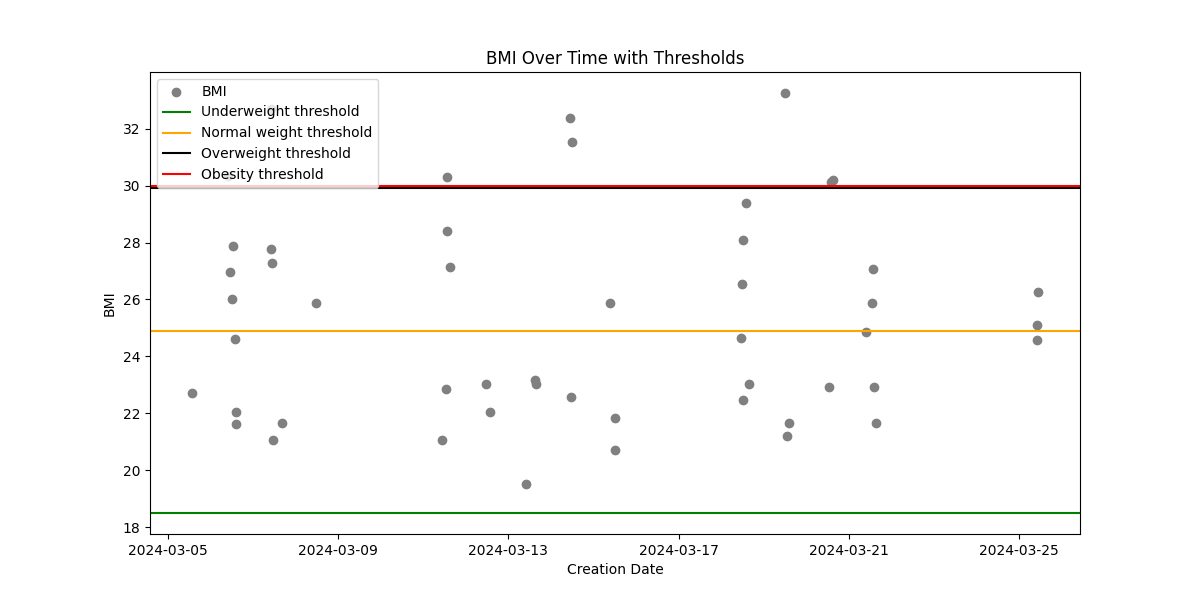
\includegraphics[width=1.0\linewidth]{Master Thesis/Plots/BMI.png}
\caption{Distribution of BMI values of all subjects}
\label{fig:distBMI}
\end{figure}
\FloatBarrier

To address the sex determination challenge, a general BMI formula was employed. The BMI values were calculated and general thresholds were plotted to categorize the subjects effectively. The plot illustrates the distribution of BMI values over time, showcasing various thresholds for underweight, normal weight, overweight, and obesity as defined by the World Health Organization (WHO).

As seen in the figure ~\ref{fig:distBMI}, none of the subjects is in the underweight category. A significant number of subjects have a BMI within the normal range. Some subjects exhibit a BMI over 25, indicating slight overweight, while a few have a BMI over 30, which is classified as unhealthy overweight according to WHO standards. This distribution provides valuable insights into the overall health status of the subjects, allowing for a better understanding of the population under study.

By integrating BMI calculations into the analysis, it becomes possible to gain a more comprehensive view of the subjects' health metrics, going beyond simple feature-based categorization. This approach underscores the importance of utilizing multiple health indicators to achieve more accurate and informative results. The use of BMI as an additional metric provides a clearer picture of the health and fitness levels of the subjects, which is crucial for making more informed conclusions and recommendations.

\section{Cross Entropy of the Study Dataset}

For getting a even better insight into our data, we calculated the cross entropy for the most important features of our work. Cross entropy is a key concept in information theory used to measure the difference between two probability distributions. When comparing two distributions, cross entropy quantifies the amount of additional information required to describe one distribution using another. This measurement is especially useful for analyzing how one set of values diverges from another, offering insights into their similarity or dissimilarity. By calculating cross entropy, we can better understand the distributional characteristics of different datasets, which is essential for various applications in statistics and data analysis.

For the feature heart rate, we obtained a cross entropy value of 0.98. This relatively low value indicates that the heart rate distributions between males and females are quite similar, as shown in the following plot:

\FloatBarrier
\begin{figure}[h!]
\centering
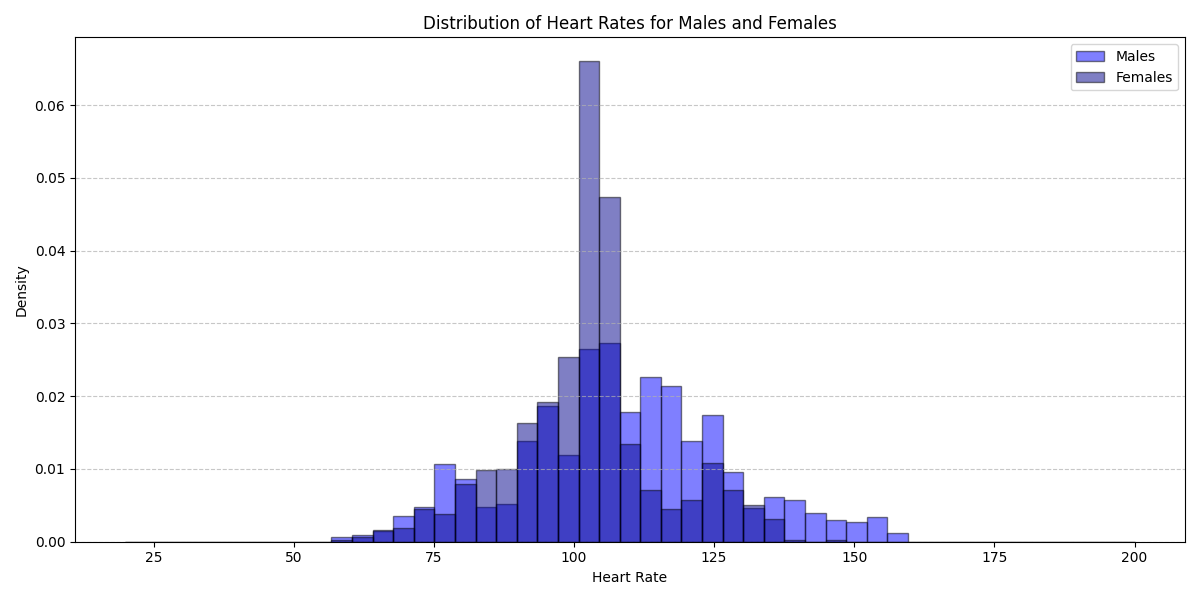
\includegraphics[width=1.0\linewidth]{Master Thesis/Plots/Dist_HeartRate_Males_Females.png}
\caption{Distribution of heart rates for males and females}
\label{fig:crossHeart}
\end{figure}
\FloatBarrier

In figure ~\ref{fig:crossHeart}, the distribution of heart rates for both male and female subjects is depicted. The plot shows that both distributions follow a similar pattern, with most heart rates clustering around 75 to 100 bpm. The peak of the male distribution is slightly higher than that of the female distribution, indicating a marginally higher heart rate in males. However, the overlap between the distributions suggests that heart rate behaviors are generally similar between sex.

The cross entropy between male and female active energy burned is 9.85, suggesting a significant difference in the distribution of active energy expenditure between the sex. The following plot illustrates these differences:

\FloatBarrier
\begin{figure}[h!]
\centering
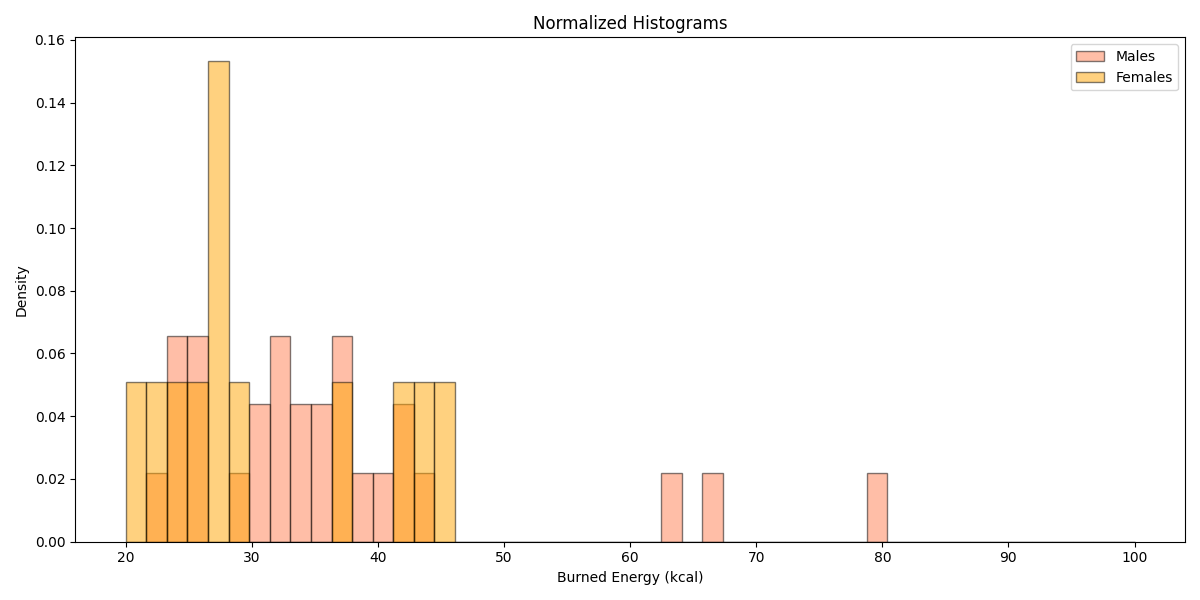
\includegraphics[width=1.0\linewidth]{Master Thesis/Plots/CrossEntro_ActiveEnergyBurned_all.png}
\caption{Distribution of active energy burned for males and females}
\label{fig:distActBurn}
\end{figure}
\FloatBarrier

Figure ~\ref{fig:distActBurn} illustrates the distribution of active energy burned for males and females. The plot reveals noticeable differences, with males generally burning more active energy compared to females. The male distribution shows a peak around 40 to 50 kcal, while the female distribution peaks around 20 to 30 kcal. This indicates that males tend to engage in more intense physical activities that burn higher amounts of energy.

For the basal energy burned, the cross entropy value is 19.49, indicating a considerable divergence between the distributions for males and females. This is depicted in the following plot:

\FloatBarrier
\begin{figure}[h!]
\centering
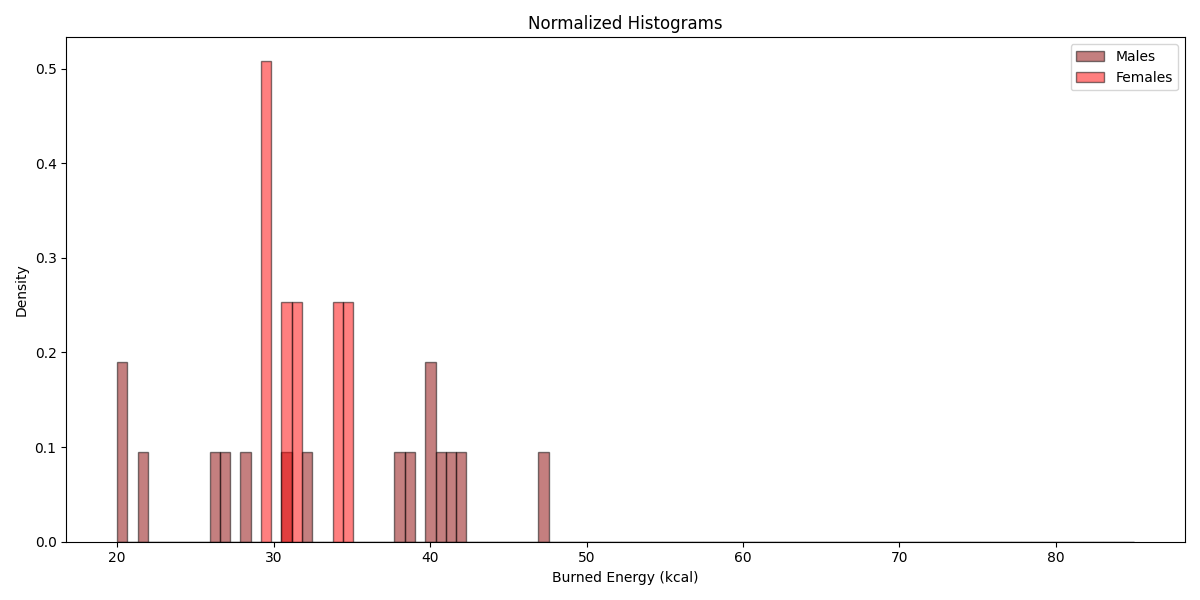
\includegraphics[width=1.0\linewidth]{Master Thesis/Plots/CrossEntro_BasalEnergyBurned_all.png}
\caption{Distribution of basal energy burned for males and females}
\label{fig:Distbasburn}
\end{figure}
\FloatBarrier

In figure ~\ref{fig:Distbasburn}, the distribution of basal energy burned during the recorded movement session is shown for both sex. The plot shows a clear divergence, with males generally burning more basal energy than females. The male distribution peaks around 1500 to 2000 kcal, while the female distribution peaks around 1000 to 1500 kcal. This significant difference reflects the higher basal metabolic rate in males, which is consistent with physiological differences between sex.

Regarding the walked distance, we achieved a cross entropy value of 8.46. This value suggests a moderate difference in the distribution of walked distances between males and females, as illustrated in the following plot:

\FloatBarrier
\begin{figure}[h!]
\centering
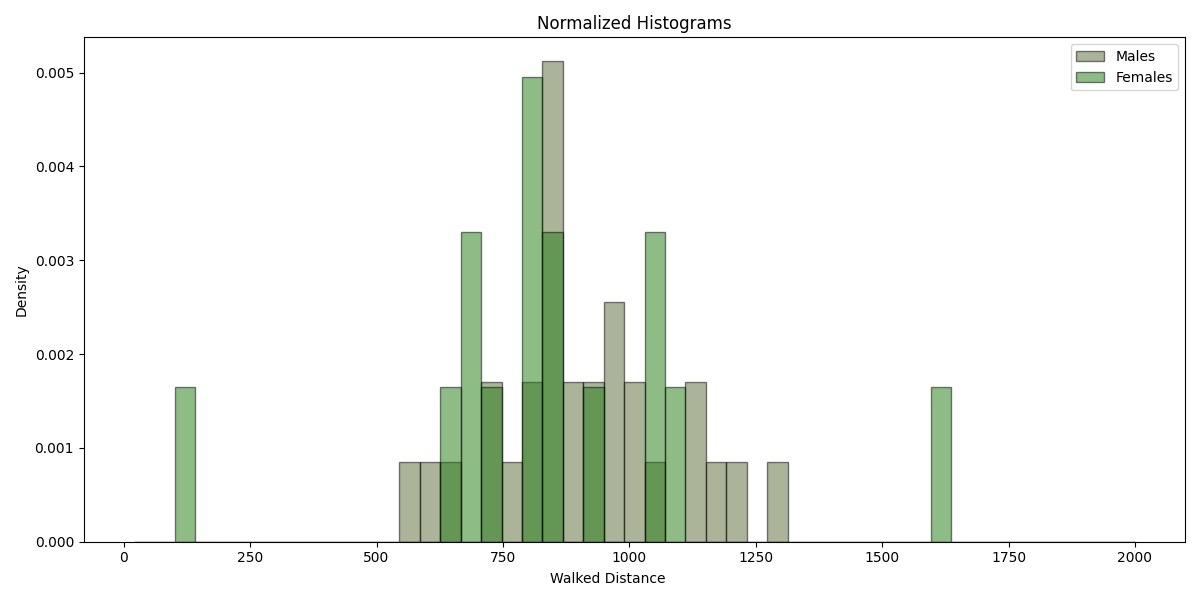
\includegraphics[width=1.0\linewidth]{Master Thesis/Plots/CrossEntro_Distance_all.jpeg}
\caption{Distribution of walked distances for males and females}
\label{fig:distWalkedRun}
\end{figure}
\FloatBarrier

Figure ~\ref{fig:distWalkedRun} displays the distribution of walked distances in meters for males and females. The plot shows that males tend to walk slightly longer distances than females. The male distribution has a peak around 1000 m, while the female distribution shows a peak around 750 m. However, the overall distribution is relatively similar between the two sex, indicating that walking distance is a more uniform activity across sex compared to energy expenditure metrics.

These cross entropy values provide valuable insights into the differences and similarities in health metrics between male and female subjects within the study dataset. Understanding these divergences helps to inform further analysis and applications in the field of health data analysis.

\newpage

We have now described the process of data extraction and preparation in detail. We have focused on the critical aspects of the study dataset. We described the methods used to convert XML files into CSV tables, the selection and merging of relevant data from different sources, and the specific criteria used to ensure the accuracy and completeness of the dataset. We also explained the rationale for selecting certain characteristics and metrics, such as heart rate values and BMI calculations, to provide a comprehensive basis for our analysis.